
\documentclass[]{article}
\usepackage[margin=1in]{geometry}
\usepackage{tikz}
\usetikzlibrary{calc,intersections}

\begin{document}
	
\begin{minipage}{0.33\linewidth}
	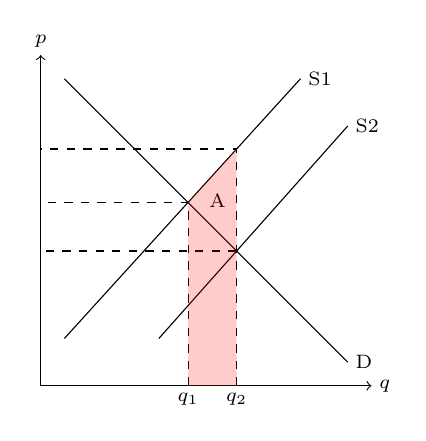
\begin{tikzpicture}[scale=0.6]
	\scriptsize
	\draw[<->] (0,7)node[above]{$p$}--(0,0)--(7,0) node[right]{$q$};
	\draw[name path = D1] (0.5,6.5)--(6.5,0.5) node[right]{D};	
	\draw[name path = S2] (2.5,1)--(6.5,5.5) node[right]{S2};
	\draw[name path = S1] (0.5,1)--(5.5,6.5) node[right]{S1};	
	
	\draw[dashed, name intersections={of=D1 and S1}, name path = I1] let \p1 = (intersection-1) in (\x1,0) node[below]{$q_1$}--(\x1,\y1)--(0,\y1) coordinate(B) at (\x1,\y1);
	\draw[dashed, name intersections={of=D1 and S2}, draw opacity = 0, name path = I2] let \p1 = (intersection-1) in (\x1,0)--(\x1,7);
	\draw[dashed, name intersections={of=D1 and S2}] let \p1 = (intersection-1) in (\x1,\y1)--(0,\y1) coordinate(C) at (\x1,\y1);
	\draw[dashed, name intersections={of=I2 and S1}] let \p1 = (intersection-1) in (\x1,0) node[below]{$q_2$}--(\x1,\y1)--(0,\y1) coordinate(A) at (\x1,\y1);
	
	\node at (barycentric cs:A=1,B=1.3,C=1) {A};
	\coordinate(O) at (0,0);
	
	\fill[red, fill opacity = 0.2] (B|-O)--(B)--(A)--(A|-O);
	\end{tikzpicture}
\end{minipage}
\begin{minipage}{0.33\linewidth}
	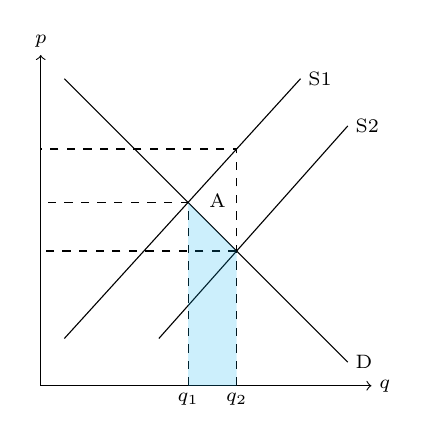
\begin{tikzpicture}[scale=0.6]
	\scriptsize
	\draw[<->] (0,7)node[above]{$p$}--(0,0)--(7,0) node[right]{$q$};
	\draw[name path = D1] (0.5,6.5)--(6.5,0.5) node[right]{D};	
	\draw[name path = S2] (2.5,1)--(6.5,5.5) node[right]{S2};
	\draw[name path = S1] (0.5,1)--(5.5,6.5) node[right]{S1};	
	
	\draw[dashed, name intersections={of=D1 and S1}, name path = I1] let \p1 = (intersection-1) in (\x1,0) node[below]{$q_1$}--(\x1,\y1)--(0,\y1) coordinate(B) at (\x1,\y1);
	\draw[dashed, name intersections={of=D1 and S2}, draw opacity = 0, name path = I2] let \p1 = (intersection-1) in (\x1,0)--(\x1,7);
	\draw[dashed, name intersections={of=D1 and S2}] let \p1 = (intersection-1) in (\x1,\y1)--(0,\y1) coordinate(C) at (\x1,\y1);
	\draw[dashed, name intersections={of=I2 and S1}] let \p1 = (intersection-1) in (\x1,0) node[below]{$q_2$}--(\x1,\y1)--(0,\y1) coordinate(A) at (\x1,\y1);
	
	
	\node at (barycentric cs:A=1,B=1.3,C=1) {A};
	\coordinate(O) at (0,0);
	
	\fill[cyan, fill opacity = 0.2] (B|-O)--(B)--(C)--(C|-O);
	\end{tikzpicture}
\end{minipage}
\begin{minipage}{0.33\linewidth}
	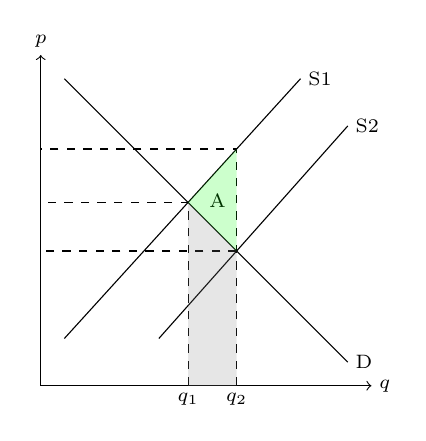
\begin{tikzpicture}[scale=0.6]
	\scriptsize
	\draw[<->] (0,7)node[above]{$p$}--(0,0)--(7,0) node[right]{$q$};
	\draw[name path = D1] (0.5,6.5)--(6.5,0.5) node[right]{D};	
	\draw[name path = S2] (2.5,1)--(6.5,5.5) node[right]{S2};
	\draw[name path = S1] (0.5,1)--(5.5,6.5) node[right]{S1};	
	
	\draw[dashed, name intersections={of=D1 and S1}, name path = I1] let \p1 = (intersection-1) in (\x1,0) node[below]{$q_1$}--(\x1,\y1)--(0,\y1) coordinate(B) at (\x1,\y1);
	\draw[dashed, name intersections={of=D1 and S2}, draw opacity = 0, name path = I2] let \p1 = (intersection-1) in (\x1,0)--(\x1,7);
	\draw[dashed, name intersections={of=D1 and S2}] let \p1 = (intersection-1) in (\x1,\y1)--(0,\y1) coordinate(C) at (\x1,\y1);
	\draw[dashed, name intersections={of=I2 and S1}] let \p1 = (intersection-1) in (\x1,0) node[below]{$q_2$}--(\x1,\y1)--(0,\y1) coordinate(A) at (\x1,\y1);
	
	
	\node at (barycentric cs:A=1,B=1.3,C=1) {A};
	\coordinate(O) at (0,0);
	
	\fill[gray, fill opacity = 0.2] (B|-O)--(B)--(C)--(C|-O);
	\fill[green, fill opacity = 0.2] (A)--(B)--(C);
	\end{tikzpicture}
\end{minipage}

\textbf{}\\

\begin{minipage}{0.33\linewidth}
	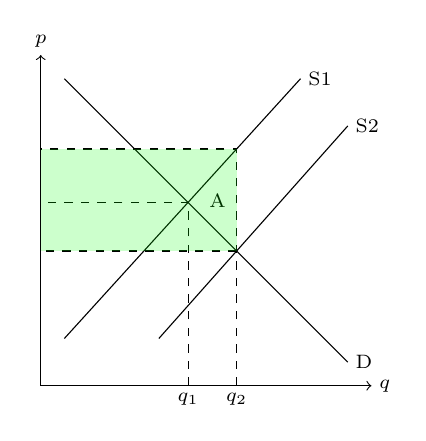
\begin{tikzpicture}[scale=0.6]
	\scriptsize
	\draw[<->] (0,7)node[above]{$p$}--(0,0)--(7,0) node[right]{$q$};
	\draw[name path = D1] (0.5,6.5)--(6.5,0.5) node[right]{D};	
	\draw[name path = S2] (2.5,1)--(6.5,5.5) node[right]{S2};
	\draw[name path = S1] (0.5,1)--(5.5,6.5) node[right]{S1};	
	
	\draw[dashed, name intersections={of=D1 and S1}, name path = I1] let \p1 = (intersection-1) in (\x1,0) node[below]{$q_1$}--(\x1,\y1)--(0,\y1) coordinate(B) at (\x1,\y1);
	\draw[dashed, name intersections={of=D1 and S2}, draw opacity = 0, name path = I2] let \p1 = (intersection-1) in (\x1,0)--(\x1,7);
	\draw[dashed, name intersections={of=D1 and S2}] let \p1 = (intersection-1) in (\x1,\y1)--(0,\y1) coordinate(C) at (\x1,\y1);
	\draw[dashed, name intersections={of=I2 and S1}] let \p1 = (intersection-1) in (\x1,0) node[below]{$q_2$}--(\x1,\y1)--(0,\y1) coordinate(A) at (\x1,\y1);
	
	
	\node at (barycentric cs:A=1,B=1.3,C=1) {A};
	\coordinate(O) at (0,0);
	
	\fill[green, fill opacity = 0.2] (C-|O) rectangle (A);
	\end{tikzpicture}
\end{minipage}
\begin{minipage}{0.33\linewidth}
	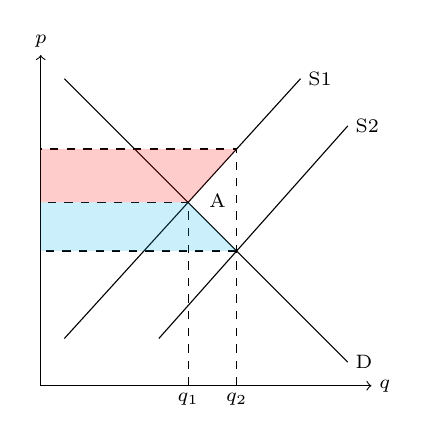
\begin{tikzpicture}[scale=0.6]
	\scriptsize
	\draw[<->] (0,7)node[above]{$p$}--(0,0)--(7,0) node[right]{$q$};
	\draw[name path = D1] (0.5,6.5)--(6.5,0.5) node[right]{D};	
	\draw[name path = S2] (2.5,1)--(6.5,5.5) node[right]{S2};
	\draw[name path = S1] (0.5,1)--(5.5,6.5) node[right]{S1};	
	
	\draw[dashed, name intersections={of=D1 and S1}, name path = I1] let \p1 = (intersection-1) in (\x1,0) node[below]{$q_1$}--(\x1,\y1)--(0,\y1) coordinate(B) at (\x1,\y1);
	\draw[dashed, name intersections={of=D1 and S2}, draw opacity = 0, name path = I2] let \p1 = (intersection-1) in (\x1,0)--(\x1,7);
	\draw[dashed, name intersections={of=D1 and S2}] let \p1 = (intersection-1) in (\x1,\y1)--(0,\y1) coordinate(C) at (\x1,\y1);
	\draw[dashed, name intersections={of=I2 and S1}] let \p1 = (intersection-1) in (\x1,0) node[below]{$q_2$}--(\x1,\y1)--(0,\y1) coordinate(A) at (\x1,\y1);
	
	
	\node at (barycentric cs:A=1,B=1.3,C=1) {A};
	\coordinate(O) at (0,0);
	
	\fill[red, fill opacity = 0.2] (B-|O)--(B)--(A)--(A-|O);
	\fill[cyan, fill opacity = 0.2] (B-|O)--(B)--(C)--(C-|O);
	
	\end{tikzpicture}
\end{minipage}
\begin{minipage}{0.33\linewidth}
	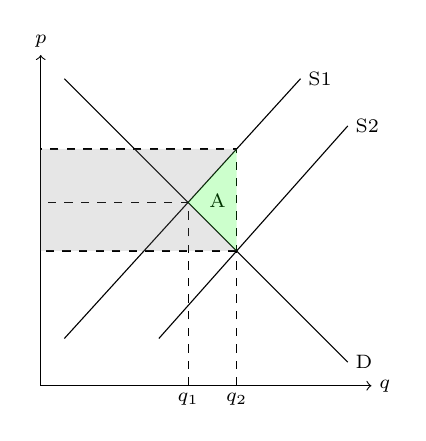
\begin{tikzpicture}[scale=0.6]
	\scriptsize
	\draw[<->] (0,7)node[above]{$p$}--(0,0)--(7,0) node[right]{$q$};
	\draw[name path = D1] (0.5,6.5)--(6.5,0.5) node[right]{D};	
	\draw[name path = S2] (2.5,1)--(6.5,5.5) node[right]{S2};
	\draw[name path = S1] (0.5,1)--(5.5,6.5) node[right]{S1};	
	
	\draw[dashed, name intersections={of=D1 and S1}, name path = I1] let \p1 = (intersection-1) in (\x1,0) node[below]{$q_1$}--(\x1,\y1)--(0,\y1) coordinate(B) at (\x1,\y1);
	\draw[dashed, name intersections={of=D1 and S2}, draw opacity = 0, name path = I2] let \p1 = (intersection-1) in (\x1,0)--(\x1,7);
	\draw[dashed, name intersections={of=D1 and S2}] let \p1 = (intersection-1) in (\x1,\y1)--(0,\y1) coordinate(C) at (\x1,\y1);
	\draw[dashed, name intersections={of=I2 and S1}] let \p1 = (intersection-1) in (\x1,0) node[below]{$q_2$}--(\x1,\y1)--(0,\y1) coordinate(A) at (\x1,\y1);
	
	
	\node at (barycentric cs:A=1,B=1.3,C=1) {A};
	\coordinate(O) at (0,0);
	
	\fill[gray, fill opacity = 0.2] (B-|O)--(B)--(A)--(A-|O);
	\fill[gray, fill opacity = 0.2] (B-|O)--(B)--(C)--(C-|O);
	\fill[green, fill opacity = 0.2] (A)--(B)--(C);
	\end{tikzpicture}
\end{minipage}

\end{document}